\chapter{Overview} % Main chapter title

\label{Chapter3} % Change X to a consecutive number; for referencing this chapter elsewhere, use \ref{ChapterX}

\lhead{Capitolo 3. \emph{Overview della soluzione}} % Change X to a consecutive number; this is for the header on each page - perhaps a shortened title

\begin{figure}[htbp]
	\centering
		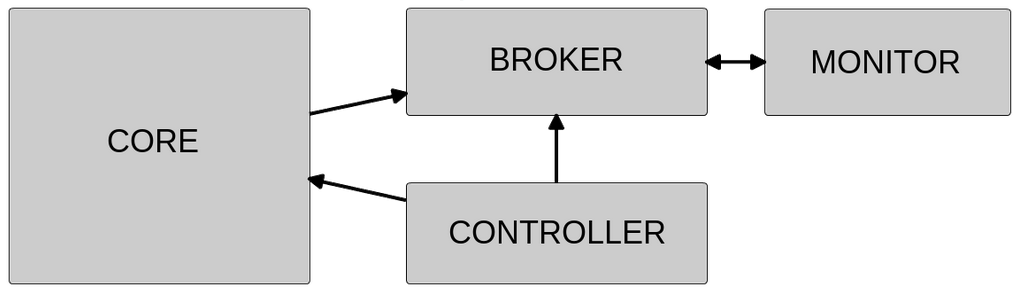
\includegraphics[keepaspectratio = true, width = 400px] {Pictures/nodes}
		\rule{35em}{0.5pt}
	\caption[Struttura]{Struttura ad alto livello.}
	\label{fig:Struttura}
\end{figure}

Come si può vedere dall’immagine, l’architettura del simulatore è stata diviso in quattro parti:
\begin{itemize}
 \item \textbf{Core}: esegue la simulazione vera e propria, calcolando i tempi, le velocità e tutto ciò che è necessario per lo svolgimento della gara
 \item \textbf{Broker}: riceve gli eventi riguardanti lo svolgimento della gara, li elabora, e li distribuisce agli elementi che ne permettono la visualizzazione ed il controllo da parte dell’utente
 \item \textbf{Monitor}: permette di visualizzare l’andamento della gara tramite una classifica ed una rappresentazione grafica dell’andamento della gara.
 \item \textbf{Controller}: dà la possibilità all’utente di agire come se fosse ai box, indicando al pilota di un veicolo che strategia utilizzare, e pianificando i pit-stop. Permette inoltre di visualizzare dati aggiuntivi sul veicolo.
\end{itemize}